
% Author: Charlie Albright, Spencer Kaiser, Luke Oglesbee
% Creation Date: 9 October 2014
% Version: 1.0
%
\documentclass{sigcomm-alternate}
\usepackage{cite}
\usepackage{fancybox}
\usepackage{pseudocode}
\usepackage{pgfplots}

\title{
Error Correction Coding in Passive UHF Gen2 Communications\\
{\large CSE 4344}
}

\numberofauthors{3}
\author{
\alignauthor Charlie A. Albright\\
\affaddr{Computer Science and Engineering Department\\
 	Southern Methodist University\\
	Dallas, Texas USA}\\
\email{calbright@smu.edu}
%
\alignauthor Spencer A. Kaiser\\
\affaddr{Computer Science and Engineering Department\\
 	Southern Methodist University\\
	Dallas, Texas USA}\\
\email{skaiser@smu.edu}
%
\alignauthor Luke W. Oglesbee\\
\affaddr{Computer Science and Engineering Department\\
 	Southern Methodist University\\
	Dallas, Texas USA}\\
\email{loglesbee@smu.edu}
}

\begin{document}

\maketitle

\section{Introduction}
The purpose of this study is to explore possible error-correcting alternatives to the simple Cyclic Redundancy Check (CRC) codes used in Ultra-High Frequency (UHF) Gen2 RFID communications. We will evaluate the complexity added to the RFID system when using various types of error-correcting codes and analyze their effects on the performance of the system. We will also compute the additional circuitry needed to implement our alternatives to CRC, and then weigh the benefits and cost of implementing this particular Error-Correcting Code (ECC) into RFID communications.

As of current, RFID uses an appended series of Cyclic Redundancy Check (CRC) bits to detect errors that happen when the information is transmitted wirelessly from Tag to Reader and from Reader to Tag. However, even if these errors are detected, the system is not able to correct the error, so the result is thrown out and another request for the Tag's ID is made. We propose that if the RFID system was able to correct one-bit or even multiple-bit errors, RFID's reliability and overall success would benefit significantly. By having an error-correcting system implemented, the Reader would be able to identify the Tag in less reads on average, and it would potentially improve the range at which the Reader could identify the Tag.

While introducing a wide variety of benefits to the system, utilizing an Error-Correcting Code will most likely increase circuit complexity and, more importantly, will increase the overall bit-length of each packet. This increased length increases the likelihood that one or more bits will flip in the presence of noise. If enough bits are flipped by noise, it is possible that the ECC will be unable to correct the packet, nullifying any potential benefit gained from its use. 

\section{Previous Work}
In their article, A New Ultralightweight RFID Authentication Protocol with Permutation, authors Tian, Chen, and Li propose implementing a strong but relatively simple protocol that implements permutation in order to establish authenticity between Reader and Tag\cite{3}. The last messages exchanged in their protocol are sent again by the reader to resist against desynchronization attacks.

Authors Grzegorz Smietanka, Jan Geldmacher and Jurgen Gotze proposed the implementation of Forward Error Correction (FEC) in their article, Error Detection Based on Correlation Analysis for BCH Encoded UHF RFID Communication\cite{1}. They say the FEC could be implemented easily because of BCH code?s similarity to CRC. 

A Secure RFID Authentication Protocol Adopting Error Correction Code talks about using a one-way hash to establish authenticity and prevent intentional transmission manipulation, which CRC is not capable of detecting. By hashing the Tag's ID, a secret key, and random challenge numbers, the authors claim that mutual authentication can be achieved\cite{5}.

Another lightweight protocol for de-synchronization is proposed by authors Zhou, Zhang, Luo, and Wong in their article A lightweight anti-desynchronization RFID authentication protocol. They claim that using the one-way hash and XOR functions while the backend server keeps a history of all shared secret keys prevents desynchronization and is capable of finding intentional errors \cite{4}.

Finally, On Error Performance Improvements of Passive UHF RFID Systems via Syndrome Decoding discusses using the existing CRC error detection implementation to correct single bit errors. Using a lookup table with various CRC codes and other information stored in it, CRC becomes capable of correcting single bit errors\cite{2}.

\section{Methodology}
In order to test the effects of adding an error-correcting code in place of the CRC which is already being utilized in RFID communications, we decided to implement a virtual testing environment. We put considerable time and thought into carefully choosing which language to implement our environment in, and after weighing the pros and cons, we chose to write our testing modules in Python due to its power and simplicity. We felt that Python's unique functionality, incredibly effective string manipulation methods, and overall lightweight qualities would be well suited for rapid processing of simulated transmissions.

Using Python, we will be able to simulate packet generation, packet encoding, and packet decoding with a high degree of consistency and accuracy. We will use random number generation to create base-packets consisting of Protocol Control Bits and an Electronic Product Code (EPC) bits then encode that packet with CRC bits and ECC bits. We will then be able to use those encoded packets to test our decode functions; if every packet can be decoded without error, we will have a high degree of confidence in our encode and decode functions for each model.

At this point we will be able to start running an analysis of our CRC and ECC decoded packets. During our analysis, we will pass these packets to one of three noise functions representing three unique noise
models. These noise models will move through each packet on a bit-level, randomly flipping bits based on a predetermined noise probability. After moving through the entire packet, we will attempt to decode the packet. 

Depending on our predetermined noise probability, it is entirely likely that a packet will be unaffected by noise. In this situation, all of our models, including CRC, will be able to successfully decode the packet and no retransmissions will be necessary. On the other hand, if the noise probability is high enough, one or more packets may be flipped. If one or more bits is flipped, the CRC function should detect an error and a retransmission will be made. The ECC functions, however, should be able to detect the errors and correct a significant number of the noise affected packets.

Once this initial implementation is complete, we will run a thorough analysis pitting the CRC packets and the ECC packets against the aforementioned noise models. During this analysis, we will continually modify a number of variables affecting the noise and decode functions and maintain statistics of how these changes impact the number of retransmissions required by each type of packet. We will also maintain statistics regarding the amount of corrections made by each type of ECC and the number of times each ECC was unable to correct a packet.

\section{Implementation and Testing}
As mentioned in the previous section, we determined that utilizing the Python programming language would allow us to effectively simulate the effects of using Cyclic Redundancy Check (CRC) versus three Error-Correcting Codes (ECC) while maintaining the greatest degree of consistency. Python features a variety of string manipulation functions which allow us to easily simulate the bit-level operations needed in each model's encode and decode functions. Similarly, these bit-level operations are necessary for each noise model's ability to flip a bit or series of bits based on a randomly generated number and a predetermined noise probability.

Our implementation is composed of a single main file which functions as a hub, importing a number of individual Python modules representing our implementation of CRC, three ECC models, and three noise models. Each of these modules is accessed by calling functions which either encode, decode, or add noise to a packet and return a result to the hub.

The "main" function in this hub file acts as the primary simulation of an RFID reader unit. This function starts by opening a text file containing one thousand randomly-generated strings of bits representing the Protocol Control Bits and Electronic Product Code (EPC) bits for individual packets. The testing environment begins by initializing a variety of variables intended to monitor the total number of packets transmitted for each model, the number of necessary retransmissions for each model, and, in the case of ECCs, the number of packets that were successfully corrected by each model. It then prepares each partial packet for analysis by stripping excess data and ensuring it fits the required length.

 At this point, each packet enters a series of loops, each of which represent either CRC or an ECC. Each loop begins by calling its respective model's encode function. These functions either append bits to the end of the packet, or restructure the packet and interweave bits for later use in the decoding process. Once the packet is encoded, it is passed to a noise model along with a probability indicating the likelihood that any individual bit will be flipped. After the noise model has successfully iterated through the entire packet, the result is returned. The encoded packet, which may or may not have been affected by noise, is now ready to be decoded.
 
Depending on whether CRC or an ECC was used, the decode process may or may not be able to successfully read a noise-affected packet. If the model was unable to decode the packet after this initial detection and/or correction, a retransmission must occur and the packet is sent through the noise model once again. This process continues until the packet is successfully read, at which point, the packet then enters the next loop.

\begin{pseudocode}{Packet Analysis}{Parameters}
\FOREACH Packet \in File 
	\DO
	\BEGIN
		Encode\ Packet\ with\ CRC\\
		\WHILE Transmission\ is\ not\ successful
			\DO
			\BEGIN
				Send\ Packet\ though\ Noise\ module\\
				Decode\ resulting\ Packet\ to\ check\ for\ errors\\
				\IF Errors\ Detected
					\THEN
					\BEGIN
						Retransmission\ occurs
					\END
				\ELSEIF Errors\ exist\ but\ undetected
					\THEN
					\BEGIN
						Undetected\ Error\ occurs
					\END
				\ELSE
					Successful\ transmission
			\END\\\\
		Encode\ Packet\ With\ Hamming\\
		\WHILE Transmission\ is\ not\ successful
			\DO
			\BEGIN
				Send\ Packet\ though\ Noise\ module\\
				Decode\ resulting\ Packet\ to\ check\ for\ errors\\
				\IF Errors\ Detected\ and\ Not\ Fixed
					\THEN
					\BEGIN
						Retransmission\ occurs
					\END
				\ELSEIF Errors\ exist\ but\ undetected
					\THEN
					\BEGIN
						Undetected\ Error\ occurs
					\END
				\ELSE
					Successful\ transmission
			\END
	\END\\\\
	
Print\ model\ statistics\ to\ screen
\end{pseudocode}

As previously stated, throughout this entire process the environment maintains statistics representing the total number of packets sent and received by each model and each models ability to detect and/or correct packets that were affected by noise.

The first loop each packet enters is the CRC loop. Our implementation of CRC contains two primary functions: one to encode each raw packet, and one to decode a packet that may or may not have been affected by noise.

\begin{pseudocode}{CRC}{Packet}
\PROCEDURE{Encode}{Packet}
\mbox{append 16-bit placeholder CRC bits to } Packet\\
polynomial \GETS \mbox{0x8005}\\
subPacket \GETS Packet[0:17]\\
pointer \GETS 17\\
\WHILE pointer < \mbox{length(} Packet \mbox{)}
\DO
\BEGIN
Result \GETS subPacket \mbox{ XOR } polynomial\\
subPacket \GETS Result \mbox{(w/o leading zeros)}\\
numBits \GETS \mbox{17 - length(} subPacket \mbox{)}\\
subPacket\ += Packet[pointer:pointer+numBits]\\
pointer\ += numBits
\END\\
packet \GETS Packet + subPacket\\
\RETURN {Packet}
\ENDPROCEDURE

\PROCEDURE{Decode}{Packet}
polynomial \GETS \mbox{0x8005}\\
subPacket \GETS Packet[0:17]\\
pointer \GETS 17\\
\WHILE pointer < \mbox{length(} Packet \mbox{)}
\DO
\BEGIN
Result \GETS subPacket \mbox{ XOR } polynomial\\
subPacket \GETS Result \mbox{(w/o leading zeros)}\\
numBits \GETS \mbox{17 - length(} subPacket \mbox{)}\\
subPacket\ += Packet[pointer:pointer+numBits]\\
pointer\ += numBits
\END\\
\IF subPacket \mbox{ is all zeros}
\THEN
\RETURN{True}
\ELSE
\THEN
\RETURN{False}
\ENDPROCEDURE
\end{pseudocode}

The encode function accepts a string representing a 112-bit packet. This packet is then converted into a "working packet" by appending sixteen placeholder bits to the end. It then enters the loop representing the bulk of the encode functionality. During this loop, a "sub packet" of seventeen bits is extracted from the working packet and passed through an exclusive or gate with a seventeen bit CRC polynomial. The high-order zero bits are removed and new bits are extracted from the working packet to increase the length of the sub packet until it reaches a length of seventeen bits. At this point the loop restarts, and the process continues until all the bits in the entire working packet have been added to the sub packet. At this point, the remaining contents of sub packet are padded with high order zeros to match a length of sixteen bits and appended to the original packet that was passed into the encode function. This updated packet is then returned.

The decode function operates in a very similar fashion to that of the encode function. Bits are extracted from packet passed to the function, passed into an exclusive or gate with the CRC polynomial, and new bits replace the high order zeros. This continues until all the bits from the entire packet have been pulled into the working packet. At this point, if the result is a sub packet containing all zeros, the decode was successful and a boolean True value is returned. If the remaining sub packet does not contain all zeros, an error was detected and the packet must be retransmitted. In this case, a boolean False is returned and the main file attempts to retransmit the packet.

\begin{pseudocode}{Hamming}{Signal}
	\PROCEDURE{Encode}{Signal}
		% Output \GETS [0]\\
		% ParityBits \GETS [1]\\
		% i \GETS 2\\
		\mbox{Insert empty parity bits into } Signal\\
		% \WHILE i < length(Signal) \DO
		% 	\BEGIN
		% 		\IF i \mbox{ is power of two}
		% 		\THEN
		% 			\BEGIN
		% 				ParityBits \mbox{ push } i\\
		% 				Output \mbox{ push } Signal[i]\\
		% 				i \GETS i+1\\
		% 			\END\\
		% 		\BEGIN
		% 			Output \mbox{ push } Signal[i]\\
		% 			i \GETS i+1
		% 		\END
		% 	\END\\
		\FOREACH parityBit \mbox{ in } Signal \DO
			% \BEGIN
				Signal[parityBit-1] \GETS Parity(Signal, parityBit)\\
			% \END\\
		\RETURN{Signal}
	\ENDPROCEDURE

	\PROCEDURE{Decode}{Signal}
		\FOREACH parityBit \mbox{ in } Signal \DO
			\BEGIN
				\IF Parity(Signal, parityBit) == 1
				\THEN
					ParityErrors \mbox{ push } parityBit
			\END\\
		\IF ParityErrors
		\THEN
			\BEGIN
				badBit \GETS \mbox{sum of } ParityErrrors\\
				\IF badBit \geq length(Signal)
				\THEN
					\RETURN{False}
				\ELSE
					Signal[badBit-1] \GETS !Signal[badBit-1]
			\END\\
		\mbox{Remove parity bits from } Signal\\
		\RETURN{Signal}
	\ENDPROCEDURE

	\PROCEDURE{Parity}{Signal, parityBit}
		i \GETS parityBits\\
		comp \GETS Signal[parityBits-1]\\
		\WHILE i < length(Signal) \DO
			\BEGIN
				j \GETS i\\
				\WHILE j < i+parityBit \AND j < length(Signal) \DO
					\BEGIN
						comp = comp \oplus Signal[j]\\
						j \GETS j+1
					\END\\
				i \GETS i + 2 \cdot parityBit
			\END\\
	\RETURN{comp}
	\ENDPROCEDURE
\end{pseudocode}

The Hamming module works by accepting one 112-bit simulation packet with no encoding. Since our packet is between 64 and 128 bits, the Hamming parity bits will need to be able to account for up to 128 bits, which is 2\textsuperscript{7}. Therefore, 7 parity bits are needed to encode our entire packet. The parity bits are calculated by XORing various sets of message bits to encode the Hamming bits. Once the Hamming bits are calculated, they are inserted into the packet at locations 1, 2, 4, 8, 16, 32, and 64. The packet is then returned after the encoding of the packet is complete.

Decoding the Hamming packets work in a similar fashion. The parity bits are extracted from the packet. Then, a new set of Hamming bits is calculated from the received message bits. Then, if the freshly calculated parity bits match the ones that were transmitted with the message, we know that no errors occur. However, if a single bit error occurred, the Hamming bits are used to find the specific location of the error, and then correct it. If there are errors detected, it returns a boolean false to indicate so.

\begin{pseudocode}{Gaussian Noise}{Signal, noiseRatio}
	Noise \GETS \mbox{random value (0-1) for each element of } Signal\\
	\FOR i \GETS 0 \TO length(Signal) \DO
		\BEGIN
			\IF Signal[i] < noiseRatio
			\THEN
				Signal[i] \GETS !Signal[i]
			\ELSE
				Signal[i] \GETS Signal[i]
		\END\\
	\RETURN{Signal}
\end{pseudocode}

Gaussian white noise interferes with individual bits randomly and independently. To simulate that effect, this implementation uses a simple random number generator to simulate noise. Noise in this implementation is a random number between 0 and 1 that is generated for every bit in the incoming signal. If the noise for a particular bit is below the threshold of the noise ratio, the bit is flipped. Note that in this implementation of gaussian noise small random number means that a bit is more likely to be flipped.

\begin{pseudocode}{Burst Noise}{Signal, noiseRatio, maxBitFlip=16}
	Noise \GETS \mbox{random float (0-1) for each element of } Signal\\
	Length \GETS \mbox{random int (0-maxBitFlip) for each element of } Signal\\
	i \GETS 0\\	
	\WHILE i < length(Signal) \DO
		\BEGIN
			\IF Signal[i] < noiseRatio
			\THEN
				\BEGIN
					\FOR j \GETS i \TO i+Length[i] \DO
						\BEGIN
							Signal[j] \GETS !Signal[j]
						\END\\
					i \GETS i + j\\
				\END
			\ELSE
				i \GETS i + 1
		\END\\
	\RETURN{Signal}
\end{pseudocode}

Burst Noise interferes with a series contiguous bits. The Burst Noise implementation starts off with a random noise value between 0 and 1 for every bit in the incoming signal, similar to Gaussian White Noise. In addition to the random noise value, a random length value from 0 to some max bit value (16 by default) is generated for every bit in the incoming signal. If a signal bit has a corresponding noise value that is less than the noise ratio, that single bit is not flipped, instead the next n bits are flipped, where is the random length specified above.

As we move towards our final deliverable, the main file is likely to change. We will more than likely streamline the method in which we pass each packet to each CRC or ECC function and we will incorporate all three noise models into each packet analysis cycle. In addition, we will also incorporate functionality to better graph the data in real time so we are able to fine-tune the noise probability variables used by each noise model and increase the significance of our results.

\section{Initial Findings}
Thus far our analysis indicates that the utilization of both Cyclic Redundancy Check and Error Correcting Codes have merit in RFID communications. The graph below demonstrates the retransmission rate of both CRC and the Hamming Error Correcting Code as the noise ratio increases in different noise models.

The following shows the retransmission rate of packets run through a Gaussian White Noise model and using CRC and Hemming error detection/correction. While the Hamming code has a very small increase to its retransmission rate as the noise ratio changes, CRC drastically increases to a dysfunctional level.\\

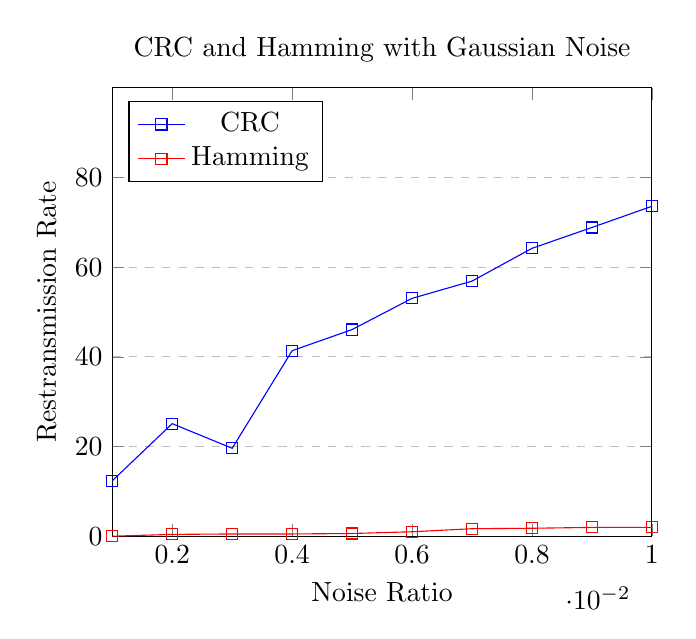
\begin{tikzpicture}
\begin{axis}[
    title={CRC and Hamming with Gaussian Noise},
    xlabel={Noise Ratio},
    ylabel={Restransmission Rate},
    xmin=0.001, xmax=0.01,
    ymin=0, ymax=100,
    xtick={0.002,0.004,0.006,0.008,0.01},
    ytick={0,20,40,60,80},
    legend pos=north west,
    ymajorgrids=true,
    grid style=dashed,
]
\addplot[
    color=blue,
    mark=square,
    ]
    coordinates {
    (0.001,12.36)(0.002,25.1)(0.003,19.61)(0.004,41.38)(0.005,46.09)
    (0.006,53.05)(0.007,56.9)(0.008,64.21)(0.009,68.86)(0.01,73.59)
    };
\addplot[
    color=red,
    mark=square,
    ]
    coordinates {
    (0.001,0)(0.002,0.4)(0.003,0.5)(0.004,0.5)(0.005,0.6)
    (0.006,0.99)(0.007,1.67)(0.008,1.77)(0.009,1.96)(0.01,1.96)
    };
    \legend{CRC, Hamming}
 
\end{axis}
\end{tikzpicture} \\


Running packets through a Burst Noise Filter provied a similar outcome to the Gaussian White Noise graph above. The number of retransmissions for packets using Hamming error correction/detection increased slowly but stayed below 2\% even up to a 0.01 noise ratio. On the contrary, the retranmission rate for packets using CRC error detection rose steeply and steeply as the noise ratio was increased.\\

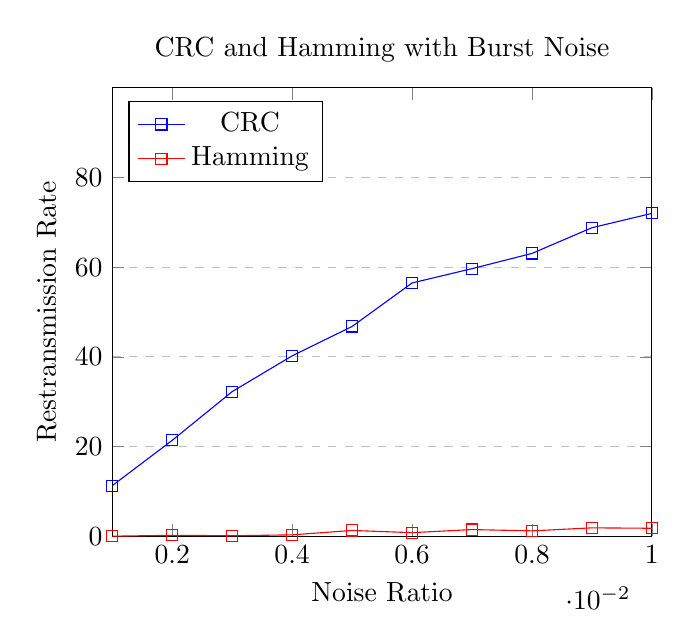
\begin{tikzpicture}
\begin{axis}[
    title={CRC and Hamming with Burst Noise},
    xlabel={Noise Ratio},
    ylabel={Restransmission Rate},
    xmin=0.001, xmax=0.01,
    ymin=0, ymax=100,
    xtick={0.002,0.004,0.006,0.008,0.01},
    ytick={0,20,40,60,80},
    legend pos=north west,
    ymajorgrids=true,
    grid style=dashed,
]
\addplot[
    color=blue,
    mark=square,
    ]
    coordinates {
    (0.001,11.27)(0.002,21.38)(0.003,32.25)(0.004,40.23)(0.005,46.78)(0.006,56.48)(0.007,59.68)(0.008,63.07)(0.009,68.81)(0.01,72.0)
    };
\addplot[
    color=red,
    mark=square,
    ]
    coordinates {
    (0.001,0.0)(0.002,0.2)(0.003,0.1)(0.004,0.3)(0.005,1.28)(0.006,0.79)(0.007,1.48)(0.008,1.19)(0.009,1.86)(0.01,1.77)
    };
\legend{CRC, Hamming}
 
\end{axis}
\end{tikzpicture} \\

Moving forward, we will complete additional analyses for CRC and each ECC model against every type of noise model. We will also attempt to graphically demonstrate the drawbacks of using ECC in limited-noise situations.

\section{Progress Report \& Road Blocks}
Since our initial proposal, we have made great progress towards our goal. We have fully implemented Cyclic Redundancy Check and the Hamming function and we have successfully integrated two of the three required noise models. We have also found a way to maintain statistics representing each model's effectiveness.

Unfortunately, we have had tremendous difficulty understanding the implementation of the Reed-Solomon error correcting code. We have spent countless hours digging into documentation regarding it's process and we have been unable to recreate it.

Similarly, we have been unable to gather any truly meaningful data regarding the number of logic gates required by CRC functionality, and thus, we have been unable to accurately determine the number of additional gates needed for each of our three ECCs. This is something we are going to have to have to spend additional time researching and we may reach out to on-campus resources for help with the matter.

Overall we feel we have made significant progress as a group and we now feel that our revised schedule is appropriate. We believe we are on track for the final deliverable and we believe we will have meaningful data from our analysis, which will accurately represent our study's findings.

\section{Revised Research Plan}

\textbf{11/11/14: Interim report Due}

11/12 - 11/16: Implement missing Noise and ECC models

11/17 - 11/21: Perform final analysis on effectiveness of each Error Correcting Code for each Noise Model and collect data for comparison

11/22 - 11/27: FINAL WORK PERIOD - Make final additions to paper and revise

11/28: Assign presentation sub-sections to team members

11/28 - 12/1: Team members individually create presentation components

12/1 - TBD: Compile final presentation from components and practice delivery

\textbf{TBD (12/2/14 - 12/4/14): Final Presentation}

\nocite{*}
\bibliographystyle{plain}
\bibliography{AlbrightKaiserOglesbeeInterimReport} 

\balancecolumns
%---- End the Document
\end{document}




